\documentclass{article}
\usepackage{minted}
\usepackage{amsmath,graphicx}
\usepackage[utf8]{inputenc}
\usepackage[icelandic]{babel}
\usepackage[T1]{fontenc}
\usepackage{epstopdf}
\usepackage{graphicx}

\title{Viðmótsforritun: Verkefni 5}
\author{Daníel Eldjárn Vilhjálmsson  \\
  Háskóli Íslands
  }



\date{9. mars 2014}
\begin{document}
\maketitle
Eftirfarandi er einfalt dagbókarforrit hannað í java. Þýða má forritið með skipuninni \textbf{ javac -cp .:jcalendar$_$1.4.jar Main.java } og keyra með \textbf{ java -cp .:jcalendar$_$1.4.jar Main }



\begin{figure}[htb]
  \centering
  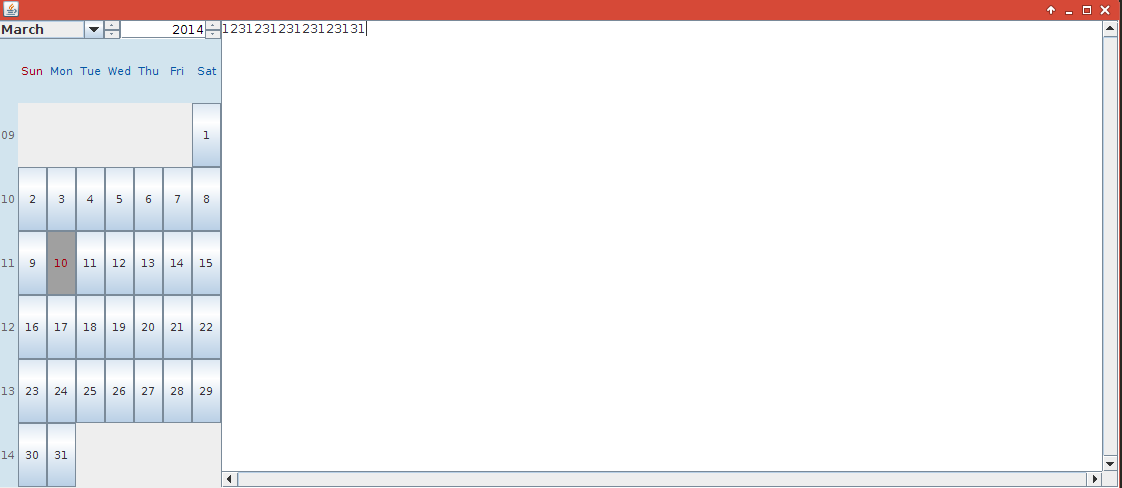
\includegraphics[width=\textwidth]{gui1.png}
  \centerline{}
  \caption{Skjáskot úr forritinu}\medskip
  \label{fig:gui}
\end{figure}

\inputminted{java}{Cal.java}
\inputminted{java}{Main.java}
\end{document}